\section{Systembeskrivelse}

\begin{figure}[H]
\centering
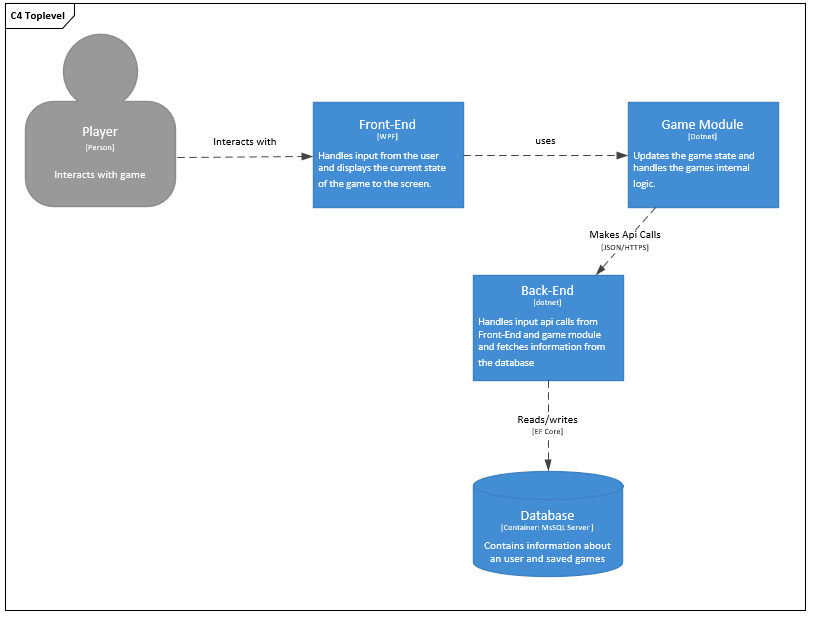
\includegraphics[width = \textwidth]{02-Body/Images/C4TopLvlDB}
\caption{C4 top level diagram, som viser kommunikation mellem systemets segmenter}
\label{fig:C4TopLvlDB}
\end{figure}

På \autoref{fig:C4TopLvlDB} ses systemets toplevel arkitektur.
Denne består af en bruger som interagerer med systemet gennem frontendapplikationen som skrives i WPF. States i denne applikation styres af Game module som holder styr på hvor spilleren befinder sig, hvilke items der er samlet op og andre nyttige information som skal bruges gennem spillet.
Spillets backend benyttes primært til bruger-authentication og som bindeled til databasen.
Databasen indeholder oplysninger om blandt andet brugere, de gemte spil og oplysninger om historien for de forskellige rum.

\newpage


\section{Kravspecifikation}
\label{sec:kravspec}

I det følgende afsnit beskrives kravene for systemet. Afsnittet indeholder et udpluk af de funktionelle og ikke funtionelle krav, som omhandler det samlede system. Til slut i afsnittet afgrænses projektets omfang her præsenteres en MoSCoW-analyse prioritering over kravene, samt hvilke rammer som sættes for projektets omfang. For en fuld kravspecifikation henvises til teknisk bilag (sektion 6).\\  


\subsection{Funktionelle krav - User Stories}
Her beskrives systemets funktionelle krav. Kravene beskrives i form af User Stories. Der er her taget udgangspunkt i User Story 1,2, 15 og 18, da disse indebærer alle systemets dele samt den mest centrale funktionalitet.\\  
 
User Story 1: Log in \\
  Som Bruger \\
  Kan jeg logge ind \\
  For at kunne se en Main Menu så jeg kan spille spillet. \\
  
User Story 2: Opret profil \\
  Som Bruger \\
  Kan jeg oprette en ny profil \\
  For at jeg kan logge ind på spillet. \\
  
UserStory 15 : Save Menu - Save Game\\
  Som bruger \\
  Kan jeg trykke på et eksisterne spil, ændre navnet og trykke "Save Game" \\
  For at gemme spillet.\\

  
UserStory 18 : Main Menu - Load Game - Load\\
  Som bruger \\
  Kan jeg trykke på "load game" \\
  For at komme ind i spillet og fortsætte med at spille det valgte spil\\


\subsection{Ikke-funktionelle krav}
Systemets ikke-funktionelle krav opstilles efter en række kategorier med inspiration fra modellen FURPS+. Igen tages her udgangspunkt i et udpluk af de ikke-funktionelle krav, som indeholder de mest kritiske punkter.\\

\textbf{DATABASE:}

\begin{itemize}

\item Skal kunne gemme maksimalt 5 save games
\item Skal kunne loade et spil indenfor maksimalt 5s
\item Skal gemme hvilke genstande man bruger lige nu
\item Skal gemme hvor meget liv man har tilbage.
\item Skal gemme hvilke fjender man har slået ihjel.
\item Skal gemme hvilke puzzles man har løst.
\item Skal gemme hvilke rum man har været i.
\end{itemize}

\textbf{GAMEPLAY:}
\begin{itemize}
\item Spillets kort skal holde styr på hvilke rum man kan komme til for et givet rum.
\item Spillets kort skal kun vise de rum som spilleren har været i.
\item Spillets kort skal, hvis spilleren har været i alle rum vise alle rum.
\item Et rum kan have maksimalt 4 forbindelser til andre rum.
\item Et rum skal have mindst 1 forbindelse til andre rum.
\item Alle Rum skal kunne nås fra ethvert andet rum, måske ikke direkte, men man skal kunne komme dertil.
\item Spillerens rygsæk skal kunne indeholde alle spillets genstande.
\item Spilleren skal have mulighed for at bruge ét våben og én rustning af gangen.
\item Spilleren skal have mulighed for at skifte hvilket våben og hvilken rustning der bruges.

\end{itemize}
    
\textbf{COMBAT:}

\begin{itemize}
\item Hvis spilleren/fjenden rammer, bliver skaden bestemt af et/flere simulerede terningekast, afhængigt af hvilket våben der bruges
\item Hvis spilleren, når nul liv inden fjenden, så dør spilleren og spillet er tabt.
\item Hvis fjenden, når nul liv inden spilleren, så dør fjenden og spilleren kan nu frit udforske rummet, som fjenden var i.
\item Hvis spilleren drikker en livseleksir bliver spillerens nuværende liv sat til fuldt.
\end{itemize}

\textbf{PERFORMANCE:}    

\begin{itemize}
\item Spillet skal respondere indenfor maksimalt 5s
\item Spillet må ikke have mere end én kommando i aktionskøen af gangen
\end{itemize}

\newpage
    

\subsection{Afgrænsning}
I dette projekt afgrænses systemet på følgende måder. Der vil ikke være fokus på at hoste systemets backend (Web API og Database) på en ekstern server. Dette er valgt for at holde fokus på selve udviklingen af systemet. Dette er noget som tages videre i det fremtidige arbejde.  

\subsubsection{MOSCOW krav}
\label{sssec:MOSCOW}
I dette afsnit er opstillet en MoSCW analyse af de krav som er opsat til projektet.\\

\textbf{MUST}
\begin{itemize}

\item have en GUI.
\item have en Database.
\item Have Netværkskommunikation.
\item Have en serie af sammenhængende rum.
\item Have et start og slut rum som ikke er det samme rum.
\item Spillet skal kunne gemmes på en Database.
\item Skal kunne hente save game fra databasen.
\item Skal have en authentication system (Accounts).
\item Hvert Rum skal bestå af et beskrivende element og en serie af actioner.
\item Spillet skal have instillinger.
\item Spillet skal have en Character.
\item Spillet skal kunne tage imod user input.
\item Spillet skal være udviklet til Windows.
\item Spillet skal være testbart i.e. skal være designet med testing in mind.

\end{itemize}


\textbf{SHOULD}
\begin{itemize}

\item Have Fjender
\item Have Items
\item Have Kamp systemer
\item Have End Screen
\item Have Character Stats
 
\end{itemize}

\textbf{COULD}

\begin{itemize}

\item Have Level development
\item Have Procedual verden
\item Have Text Parser
\item Have Sværhedsgrad
\item Have sikkerhed

\end{itemize}

\textbf{WON'T}
\begin{itemize}
\item Have Grafik
\end{itemize}

 